\documentclass[letter,10pt]{article}
\usepackage[utf8]{inputenc}
\usepackage[spanish, activeacute]{babel}
\usepackage{geometry}
\geometry{verbose,tmargin=0cm,bmargin=2cm,lmargin=2cm,rmargin=2cm,headheight=0cm,headsep=1cm,footskip=1cm}
\usepackage{graphicx}


%%%%%%%%%%%%%%%%%%%%%%%%%%%%%% Textclass specific LaTeX commands.
\newcommand{\lyxaddress}[1]{
\par {\raggedright #1
\vspace{1.4em}
\noindent\par}
}

%%%%%%%%%%%%%%%%%%%%%%%%%%%%%% User specified LaTeX commands.
\date{}

\begin{document}

\title{Problema D - Dark Souls}


\includegraphics[scale=0.6]{logo} \hspace*{9.00cm}

\includegraphics[scale=0.5]{dsc} 
\bigskip
\begin{center}
	\Large Problema D - Dark Souls
\end{center}

\begin{flushright}
Límite de tiempo: 3 segundos
\par\end{flushright}
\bigskip

\section*{Problema}

¿Alguna vez has jugado Dark Souls? ¡Se dice que es uno de los juegos más difíciles que hay!
Sus "boss fights" son casi imposibles, normalmente suele ser un enemigo enorme con muchos puntos de vida, pero cuando aparecen enemigos más chicos, aparecen en mayor cantidad e incluso puede ser mas difícil que un solo enemigo enorme. Un ejemplo de esto es cuando estás en el Valle de los Dragones y te atacan muchos al mismo tiempo. Cuando pasa esto tienes que buscar un punto ciego donde el ataque de los dragones no te alcance. En esta batalla hay dos tipos de dragones: dragones de fuego y dragones eléctricos. La forma de atacar de los dragones se ilustra en las siguientes cuadriculas.

\begin{figure}[h!]
  \begin{center}
  	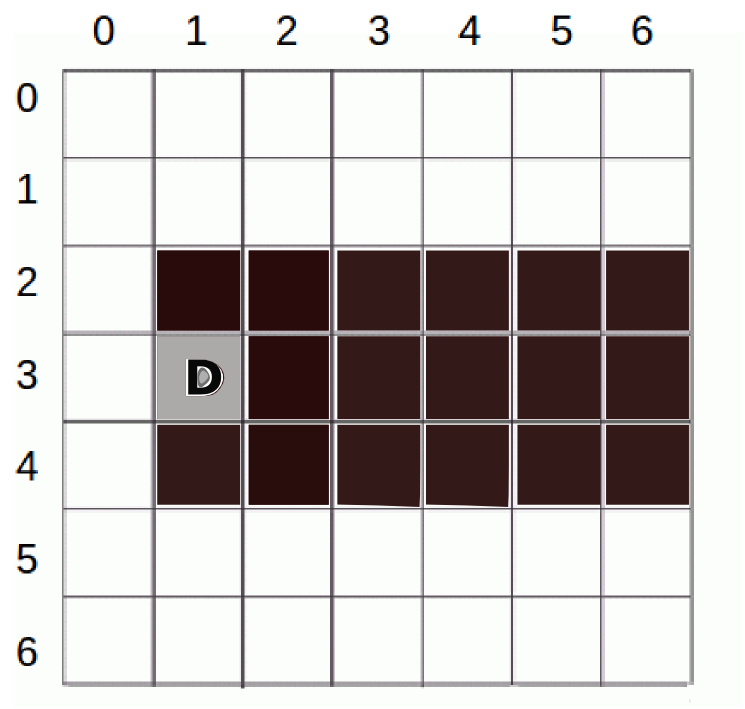
\includegraphics[scale=0.25]{dragon1}\caption{Dragon de fuego}
	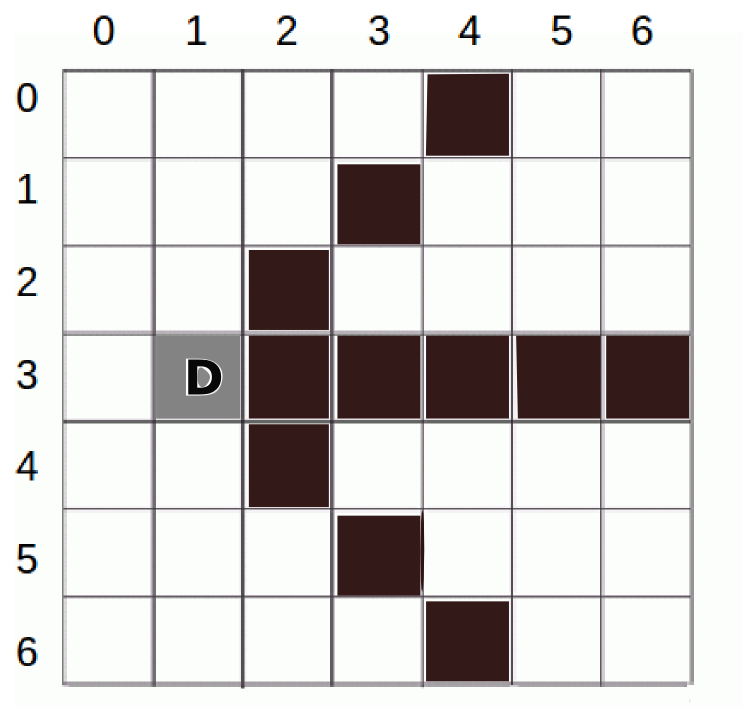
\includegraphics[scale=0.25]{dragon2}\caption{Dragon eléctrico}
  \end{center} 
\end{figure}

Los ataques se hacen en la dirección hacia donde los dragones están volteando (arriba, abajo, izquierda o derecha).

$$$$
$$$$
$$$$

Tu trabajo es, dada una cuadricula de $N \times M$, la cantidad de dragones de fuego y eléctricos y sus posiciones, encontrar si existe una casilla que no es alcanzada por los ataques. No se puede estar en la misma casilla en la que está un dragón.
\bigskip
\subsection*{Entrada}

- Un entero $T \leq 100$, el número de casos.

- Dos enteros $2 \leq N,M \leq 30$, la dimensión de la cuadrícula.

- Dos enteros $F$ y $E$, la cantidad de dragones de fuego y eléctricos respectivamente.
- Después siguen $F$ líneas y $E$ líneas con las siguientes especificaciones: Dos enteros, $X$ y $Y$ y un carácter $C$, donde $X$ y $Y$ son las coordenadas del dragón en la cuadrícula ($X$ indica en qué renglón y $Y$ indica en qué columna) y $C$ es la dirección hacia donde apunta el dragón: Arriba, Abajo, Izquierda Y Derecha, representados por los caracteres U, D, L y R respectivamente.

\subsection*{Salida}

Por cada caso de entrada se debe imprimir ``Pelear'' si existe una casilla que no es alcanzada por los ataques o imprimir ``Escapar'' en el caso contrario.

\subsection*{Entrada ejemplo}
\noindent \texttt{2}~\\
\texttt{9 9}~\\
\texttt{3 0}~\\
\texttt{0 1 D}~\\
\texttt{8 4 U}~\\
\texttt{0 7 D}~\\
\texttt{3 4}~\\
\texttt{1 2}~\\
\texttt{0 1 D}~\\
\texttt{0 0 R}~\\
\texttt{1 0 R}~\\
\noindent 

\subsection*{Salida Ejemplo}

\noindent \texttt{Escapar}~\\
\texttt{Pelear}~\\

\noindent \rule[0.5ex]{1\columnwidth}{1pt}


\lyxaddress{Hernán Tellechea Garduño - Grupo de Algorimia Avanzada y Programación Competitiva}
\end{document}
